\documentclass[../math194_paper.tex]{subfiles}

\begin{document}

\subsection{Tying Everything Together}

We can then use the following approach to determine the outcome of an endgame position
\begin{enumerate}
    \item Check that the Go position is elementary and even (\ref{parity}, \ref{elementary}).
    \item Break up the Game into independent subpositions 
    (using groups of stones that are \textit{alive}, or whose life 
    does no depend on other results).
    \item Compute the value of the chilled game for each subposition.
    \item Sum the total to determine the outcome of chilled game (Theorems \ref{addition_ordering} and \ref{linearity_cooling}).
    The outcome of the unchilled game will be the same (Theorem \ref{inverting}).
\end{enumerate}
Following \cite{berlekamp1994mathematical}, we add one extra twist to the chilled game.
For each independent subposition, add a number of markings equal to the average expected value of 
the subposition: markings equal to the full number of empty intersections for solid territory completely surrounded 
by an alive group; or markings equal to the number of empty intersections remaining after the opposing player 
attacks and the other player responds immediately to defend. 
Furthermore, stones which can be captured immediately add a marking each. \\
These are introduced for computational convenience - one could recover the same results 
by defining e.g. $* = \{-1 | 1\}$ for the position in \ref{infinitesimals}, however ``normalizing'' position values
near 0 considerably simplifies computations \cite[\S 4.1]{berlekamp1994mathematical}. 
This technique only makes sense when there an 
equal number of markings for each player, since in that case the outcome of the game is preserved.
This justifies our claim that this technique is appropriate for analyzing one-point endgames, that is endgame positions where optimal play enables a win by 1 point. \\

To find \textbf{a} a winning move for the winning player, examine 
the new sum resulting from a move on each of the subpositions. If the sum is 
still positive (resp. negative), that move is a winning move for Black 
(resp. White) - since this means that that move leads to a game with the same outcome!

\subsubsection{Corridors}
The theory can be applied to give some precise values to subpositions in the chilled version of the game - 
in addition to the subpositions for which we already computed infinitesimal values in \S \ref{infinitesimals}.
We show the proof for this first result to demonstrate how arguing on the chilled and marked game simplifies 
things.
\begin{theorem}
    \label{blocked_corridor}
    In the chilled game, a ``blocked corridor'' of length $n$ with $n-2$ markings is worth $2^{1-n}$ ($n\geq1$).
    (up to sign, depending on whether surrounding stones are Black or White).
\end{theorem}

\begin{figure}[H]
    \centering
    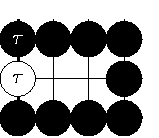
\includegraphics{figures/blocked_corridor.pdf}
    \caption*{Chilled and marked Black blocked corridor of length 2}
\end{figure}
\begin{proof}(\cite{berlekamp1991introductory}[\S 4.3]) 
We proceed by induction on a Black corridor of length $n$. For $n=1$, notice that $-1 + \int 1 = *$. \\
Now for $n \geq 2$, suppose that the value 
of the length $n$ corridor is $2^{1-n}$. A move by either player adjusts the markings on the diagram by 1. 
Note that $n+1 + \int G = \{(n + 1 )+ 1 + \int \mathcal{G}_L \mid (n+1) -1 + \int \mathcal{G}_R \}$. Then, we only 
need  to check that the resulting value for a $n+1$ corridor. A move by Black add the end 
of the corridor adds a marking and closes off the corridor, with a resulting value of $0$. On the other 
hand, a move by White at the end of the corridor yields a corridor of 
length $n$, which by hypothesis has value $2^{1-n}$. One can easily verify that the other options for each 
player are dominated by these two and ignore them by Theorem \ref{dominated}. Therefore the canonical form of 
this game is 
\[
    \{0| 2^{1-n}\} = 2^{1-(n+1)}
\]
by \ref{dyadic}, which completes the proof for Black corridors. 
The proof for a White corridor of length $n$ is obtained by taking the negation the above result.
\end{proof}

\begin{theorem}
    \label{unblocked_corridor}
    In the chilled game, an ``unblocked corridor'' of length $n$ with $n-4$ markings is worth $2^{3-n}$ ($n\geq2$)
    (up to sign, depending on whether surrounding stones are Black or White).
\end{theorem}

\begin{figure}[H]
    \centering
    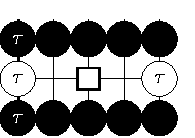
\includegraphics{figures/unblocked_corridor.pdf}
    \caption*{Chilled and marked Black unblocked corridor of length 3}
\end{figure}
The proof of this second result is similar by induction.

\subsubsection{Solving A Full Endgame Position}
\label{endgame_position}

We are now in measure to fully solve some endgame positions. The following 
example from an endgame position on a $9\times9$ board 
is adapted from \cite[\S 2]{berlekamp1994mathematical}

\begin{figure}[H]
    \centering
    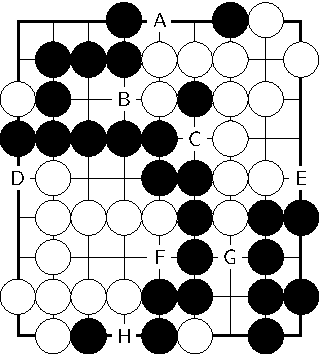
\includegraphics{figures/endgame_position.pdf}
    \caption*{White to move and win.}
\end{figure}
First, add markings for ``sure'' points of a player; and determine alive groups to check that positions $A,B,\ldots, H$
are independent.
\begin{figure}[H]
    \centering
    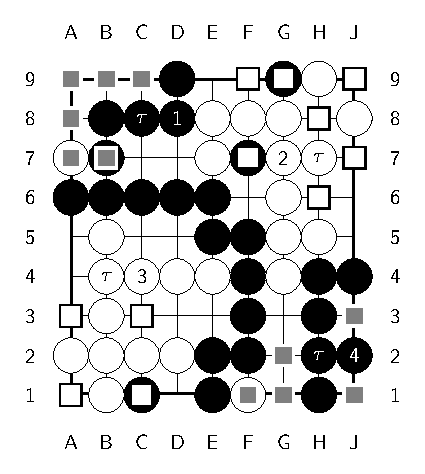
\includegraphics{figures/endgame_position_annotated.pdf}
    \caption*{Marked position with alive groups. Notice that each player has 11 markings/safe points. So 
    if suffices to gain a net advantage of one point to win (ignoring komi)}
\end{figure}
Observe that Black can guarantee two eyes for group (1) by playing, e.g. at A8, A9 or B9, and 
so group 1 is alive. \\
Next, White can guarantee life for group (2) (and other stones in the upper right corner) even if 
black attacks at J5, with a response at J6 that makes two eyes. \\
Similarly, White's group (3) can get two eyes with plays at A5, A4, D3, E3 or D1. \\
Finally, Black's group (4) already has two eyes. \\
Therefore, positions involving only these groups (and potentially isolated stones that cannot connect 
to any group other than one that is already alive), are independent from one another. Therefore, we 
can analyze the games formed by positions $A, B. \ldots H$ separately and sum to get the result 
for the full game. \\

Now, we can analyze the values of these sub-positions individually in the chilled game. Most are immediate using 
existing results:
\begin{itemize}
    \item $A = \downarrow$: this is a white corridor of length 2 with a black stone at the end 
    (\ref{basic_infinitesimals})
    \item $B = 1/2$: by Theorem \ref{blocked_corridor}, since this is a Black blocked corridor of length 2 invaded by White
    \item $C = *$: this is a black stone surrounded by White which can be captured (resp saved) in one 
    White (resp. Black) move (\ref{basic_infinitesimals})
    \item $D = -1/4$: by Theorem \ref{blocked_corridor}, since this is a White blocked corridor of length 3 invaded by White
    \item $F = -1/4$: this position is analogous to the corridor in $D$ 
    \item $G = \Uparrow *$: this is a blocked Black corridor of length 3 with a White stone at the end 
    \ref{derived_infinitesimals}
    \item $H = *$:  this is a black stone surrounded by white which can be captured (resp saved) in one 
    White (resp. Black) move (\ref{basic_infinitesimals})
\end{itemize}
$E$ requires a bit more work. On one hand, White's move a J5 dominates all of their other options, but 
adds a marking, for a net result of 0. 
On the other hand, Black's move at J5 removes a White marking, and elicits a White response at 
J6, which adds a White marking. Black surrounds no territory, while White surrounds two intersections 
but has two markings. So this position is in fact equal to $\downarrow = \{*|0\}$.  \\

Therefore, the value of this position is given by 
\[
    \underbrace{\downarrow + \downarrow + \Uparrow*}_{*} + \underbrace{1/2 - 1/4 - 1/4}_{0} +\underbrace{* + *}_{0} = *
\]
Since White plays first, they can enforce a win. Now, to find a winning move for White:
\begin{itemize}
    \item A move on $A$ at E9 changes the value from $\uparrow$ to $*$, so the sum becomes $\uparrow$, which 
    is a win for Black
    \item A move on $B$ at D2 changes the value from $-1/4$ to $0$, so the sum becomes $1/4$, which is a win for Black
    \item A move on $C$ at F6 changes the value from $*$ to $0$, so the sum becomes $0$, which is a win for White 
    (since they will play after Black)
    \item A move on $D$ at A5 changes the value from $-1/4$ to $0$, so the sum becomes $1/4$, which is a win for 
    Black
    \item A move on $E$ at J5 changes the value from $\downarrow$ to $0$, so the sum becomes $\uparrow *$, which 
    is a win for Black
    \item A move on $F$ at E3 changes the value from $-1/4$ to $0$, so the sum becomes $1/4$, which is a win 
    for Black
    \item A move on $G$ at G3 changes the value from $\Uparrow*$ to $\uparrow$, so the sum becomes $\downarrow$,
    which is a win for White
    \item A move at $H$ on D1 changes the value from $*$ to $0$, so the sum becomes $0$, which is a win for 
    White (since they will play after Black)
\end{itemize}
Therefore, winning moves for White are D1, G3 and F6. Any other move loses to Black 
(the position with value $\downarrow$ is best since $\downarrow < 0$). \\
A similar analysis can then be applied to the resulting position depending on Black's response.
To see why White wins by one point in the unchilled game, notice that if we warm the sum for the position,
\[
    \int * = \left\{ 1 + \int \{ | \} \Bigg| -1 + \int \{ | \} \right\} = \{ 1 | -1 \}
\]
So if White plays first, they get to move to $-1$, which is a win by 1 point.

Note that we did not make use of Theorem \ref{bypassing} in the above example, 
but it is frequently used to simplify a position and recover one in which we can 
apply theorems \ref{blocked_corridor} or \ref{unblocked_corridor} or one of the infinitesimals 
we defined. \\

Some more complicated positions can be analyzed using the techniques we just demonstrated, though this
can require proving several more theorems on chilled positions, one important 
example being multiple corridor invasions by one connected group. 
See \cite[\S 4]{berlekamp1994mathematical} for a more exhaustive treatment of
positions that can be solved using the theory.
\end{document}